\documentclass[a4paper, 12pt]{article}

% Set margins
\usepackage[hmargin=2cm, vmargin=2cm]{geometry}

\frenchspacing

% Language packages
\usepackage[utf8]{inputenc}
\usepackage[T1]{fontenc}
\usepackage[magyar]{babel}

% AMS
\usepackage{amssymb,amsmath}

% Graphic packages
\usepackage{graphicx}

% Colors
\usepackage{color}
\usepackage[usenames,dvipsnames]{xcolor}

% Enumeration
\usepackage{enumitem}

% C code
\usepackage{xcolor}
\usepackage{listings}

% Hyperref
\usepackage{hyperref}

\definecolor{mGreen}{rgb}{0,0.6,0}
\definecolor{mGray}{rgb}{0.5,0.5,0.5}
\definecolor{mPurple}{rgb}{0.58,0,0.82}
\definecolor{backgroundColour}{rgb}{0.95,0.95,0.92}

\lstdefinestyle{CStyle}{
    backgroundcolor=\color{backgroundColour},
    commentstyle=\color{mGreen},
    keywordstyle=\color{magenta},
    numberstyle=\tiny\color{mGray},
    stringstyle=\color{mPurple},
    basicstyle=\footnotesize,
    breakatwhitespace=false,
    breaklines=true,
    captionpos=b,
    keepspaces=true,
    numbers=left,
    numbersep=5pt,
    showspaces=false,
    showstringspaces=false,
    showtabs=false,
    tabsize=2,
    language=C
}

\title{Architektúrák, beágyazott rendszerek (GEVAU218M)\\\LARGE{\textbf{Beszámoló}}\\ \medskip \large{\textbf{ARM-SW} Szoftver fejlesztés ARM mikrovezérlőre} \\ \bigskip \LARGE{\textit{LED mátrix kijelzős óra és szöveg scroller}}}
\date{2020. december 3.}
\author{Nagy Dániel Zoltán JJ181J}

\begin{document}

\maketitle

\section{A feladat}
A féléves beadandó feladatomnak egy óra elkészítését választottam.
Az eszköz egy LED mátrix kijelzőn a pontos időt mutatja. A kijelzőn minden harmincadik másodpercben csúszó szövegkként megjelenik a napi dátum és az aktuális napnak a neve. A felhasználónak lehetősége van szöveget küldeni az eszköznek. Ezt az eszköz által szolgáltatott weboldalon teheti meg. A szöveg a kijelzőn annyiszor csúszik végig amennyiszer azt a felhasználó beállította. A weboldalon lehetőségünk van a kijelző fényerejét is konfigurálni.

\begin{figure}[ht]
	\centering
	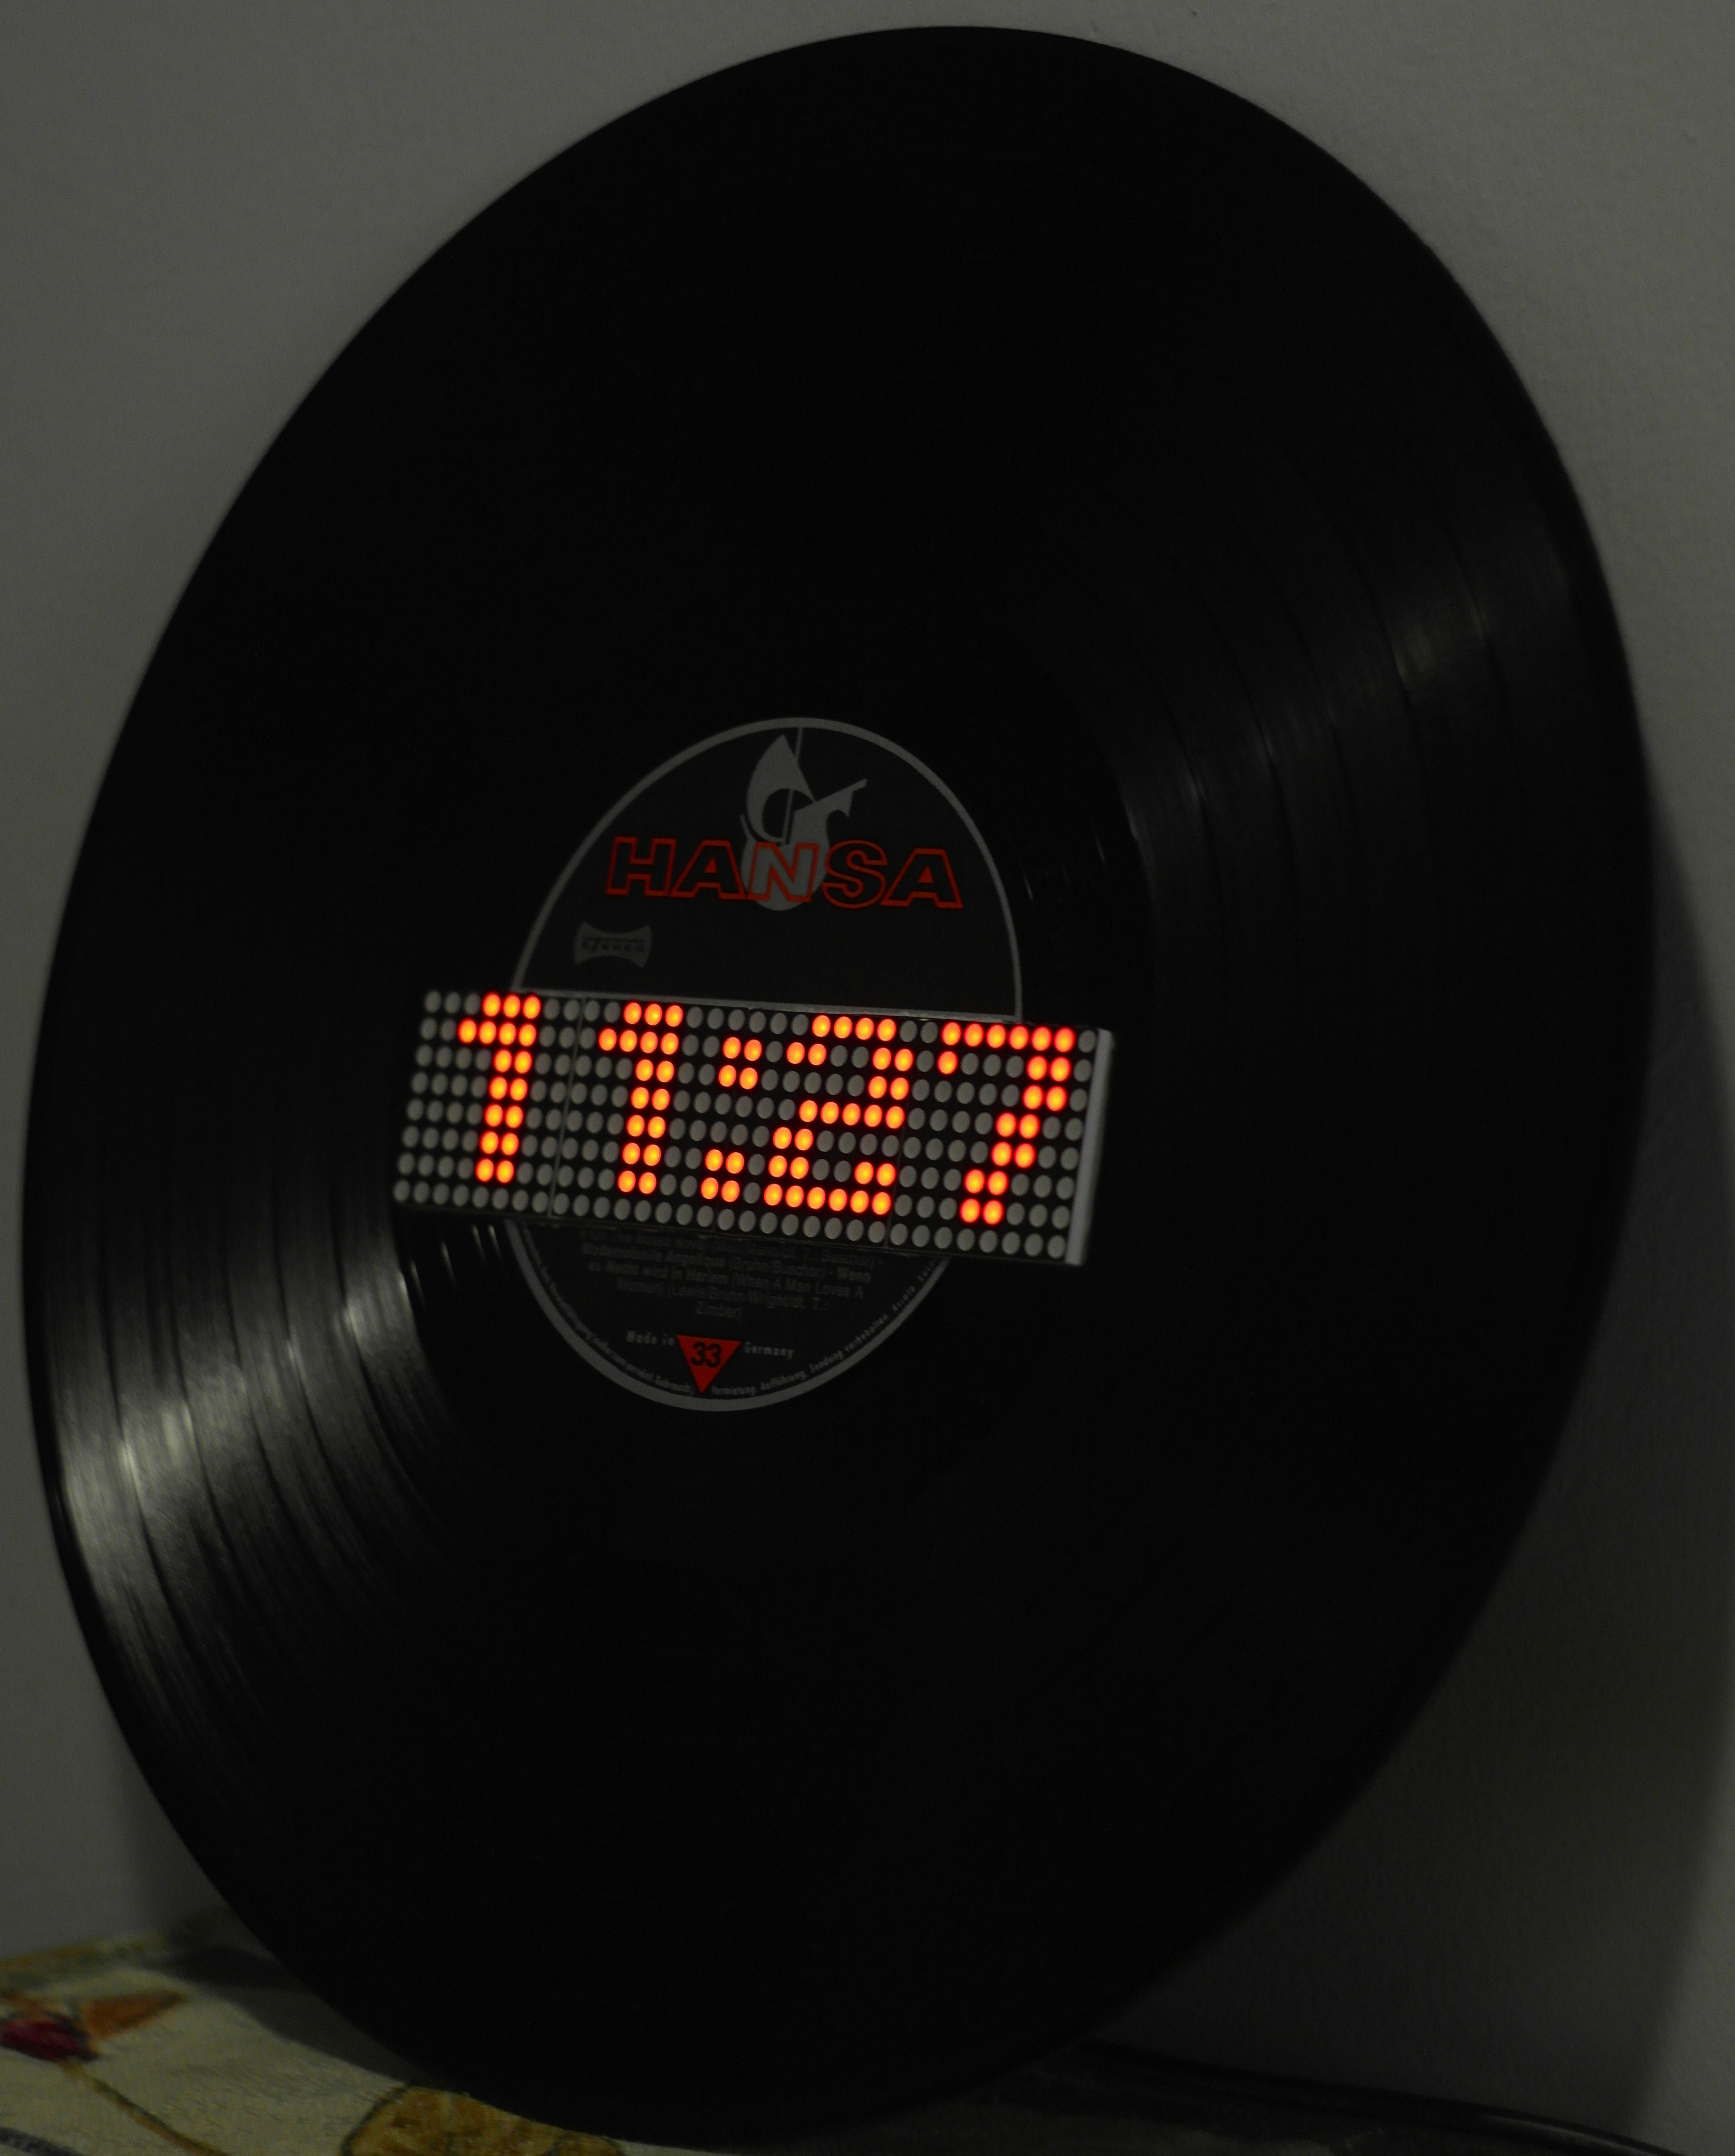
\includegraphics[width = 9cm]{images/vinyl_clock.JPG}
	\caption{Fénykép az elkészült feladatról}
	\label{fig:product}
\end{figure}	

\section{Működés}

\subsection{Megjelenítés}
Az eszköz egy mátrix kijelzőn jeleníti meg a kiírandó tartalmakat. A kijelző cellái különálló $8\times 8$-as LED mátrixok. Az egymás után fűzött cellák alkotják a kijelző felületét. A feladatomhoz 4 db cella elegendő, hiszen akkora felület tökéletesen alkalmas egy digitális óra 4 számjegyének megjelenítésére, és a csúsztatott szöveg kijelzése is megoldható vele, hiszen a 4 mátrix megfelelő szélességű felületet biztosít a szavak olasható kirajzolásához.

A szövegek megjelenítéséhez elsőként a mátrixon megjeleníthető karaktereket definiáltam. Az egyes karakterek képe leírható egy bináris kétdimenziós mátrix formájában, ahol az 1 érték világító, a 0 pedig kikapcsolt LED-et jelöl.
A karakterek dimenzióját a mátrix méretei határozzák meg. A magasság minden esetben 8 egység, a szélesség viszont változó lehet. A változó karakterszélesség használatával a szavak egybefüggőbbnek látszanak.

Példa egy G betű képére:
\begin{center}
\textbf{0 1 1 1 0\\
1 0 0 0 0\\
1 0 0 0 0\\
1 0 0 1 1\\
1 0 0 0 1\\
1 0 0 0 1\\
0 1 1 1 0\\
0 0 0 0 0}
\end{center}
A fenti példából látható, hogy a betű képét egy $5\times 8$-as bináris mátrixxal írhatjuk le. A karaktereket állítva rajzoltam meg. A legalsó sor a legtöbb esetben üres, viszont pl. a j-g-y, stb betűknél a legalsó sorban kap helyet a betű "farka".

\begin{figure}[ht]
	\centering
	\includegraphics[width = 10cm]{images/hetfo.JPG}
	\caption{Hétfő - csúszás közben}
	\label{fig:hetfo}
\end{figure}	

A karakterek azonosítása az ASCII karakterkódjaik alapján történik. Mivel nem definiáltam a teljes ASCII karakterkészletet, így bizonyos esetekben az üres helyek miatt ki kell vonni a karakterkódból a kihagyott karakterszám értékét, hogy megkapjuk a keresett karakter képének az indexét.
Ha a soron következő karakter ASCII kódja 32 és 90 közé esik, akkor 32-t kell levonni. Ha pedig 97 és 122 közé esik, akkor 38-at. A nem definiált karakterek helyett egy * képét illeszti.
Az ékezetes karakterek már nem alkotnak egybefüggő területet az ASCII kódtáblában, így hivatkozásuk egyedi értékek szerint történik.

A képernyőn megjelenő tartalom szintén egy kétdimenziós bináris mátrixalakban írható le. Méretei az egymás után összefűzött cellák által adott felületéből adódnak. Egy 4 cellából álló kijelző esetében a kijelző mérete: $32\times 8$.
A megvalósításról szóló fejezetben később kitérek arra, hogy az egyes cellák sorait egy-egy bájttal adhatjuk meg. Így a képernyőt reprezentáló mátrix oszlopainak szélessége 8 egység lesz. Vagyis egy olyan mátrixban adhatjuk meg a megjelenítendő tartalmat, amelynek 8 sora van és az oszlopok indexe az egyes cellákat jelölik, a mátrix elemei pedig 1 bájt hosszúságúak.
A megjelenítéshez ezt a nagy mátrixot kell manipulálnunk.

\subsubsection{Csúszó szöveg} \label{csuszo}
A csúszó szöveg megjelenítését a következőképpen oldottam meg:\\
Vegyünk egy $n$ karakterből álló szöveget és legyen két mutatónk: $i$, ami a soron következő karakterre mutat és $j$, amely az aktuális karakter mátrix alakjának az oszlopaira mutat. $i = 0$, $j = 0$.
A szöveget a képernyő jobboldaláról csúsztatjuk balra.
\begin{enumerate}
	\item Vegyük az szöveg $i$-edik karakterét.
	\item Az $i$-edik karakter $j$-edik oszlopát helyezzük a mátrix utolsó oszlopába.
	\item A mátrixot egy egységgel toljuk el balra. Az első egy bit szélességű oszlopa így törlődik, a jobb szélére helyezzünk egy üres, egy bit szélességű oszlopot.
	\item A mátrix képét jelenítsük meg a kijelzőn, majd várjunk $t$ időegységnyit.
	\item Növeljük a $j$ értékét eggyel, majd térjünk vissza a 2. lépésre. Egészen addig ismételjük, amíg a $j \leq$ az $i$-edik karakter képének szélességével.
	\item A mátrixot egy egységgel toljuk el balra a már ismert módon, hogy a karakterek között egy üres oszlopot hagyjunk.
	\item Növeljük az $i$ értékét eggyel, majd térjünk vissza az 1. lépésre. Egészen addig ismételjük, amíg $i \leq n$.
\end{enumerate}

A fenti eljárásban a $t$ értéke tetszőleges lehet. Minél kisebb a várakozási idő, annál gyorsabban fog a kiírandó szöveg csúszni a képernyőn.

A fenti eljárásban a harmadik lépésben megemlítem, hogy a mátrixot egy egységgel balra tolom. Az eltoláshoz figyelembe kell vennünk a szomszédos cellák értékeit.

\bigskip

\bigskip

\noindent\textbf{FOR} $k$ $\leftarrow$ 0 \textbf{TO} Hossz[képernyő] \textbf{DO}\\
\indent \textbf{FOR} $l$ $\leftarrow$ 0 \textbf{TO} 8 \textbf{DO}\\
\indent \indent \textbf{IF} $k$ = Hossz[képernyő$_l$]-1\\
\indent \indent \indent \textbf{THEN} képernyő$_{kl}$ $\leftarrow$ képernyő$_{kl}$ << 1\\
\indent \indent \textbf{ELSE}\\
\indent \indent \indent \textbf{THEN} képernyő$_{kl}$ $\leftarrow$ képernyő$_{kl}$ << 1 $\lor$ ((képernyő$_{k+1l}$ $\land$ 0x80) >> 7)

\bigskip

\bigskip
A << és >> a bitenkénti eltolás műveleteket, a $\lor$ a \textit{vagy} logikai művelet, a $\land$ pedig az \textit{és} logikai műveletet jelzi.

\newpage

\subsubsection{Az óra számlapja}

\begin{figure}[ht]
	\centering
	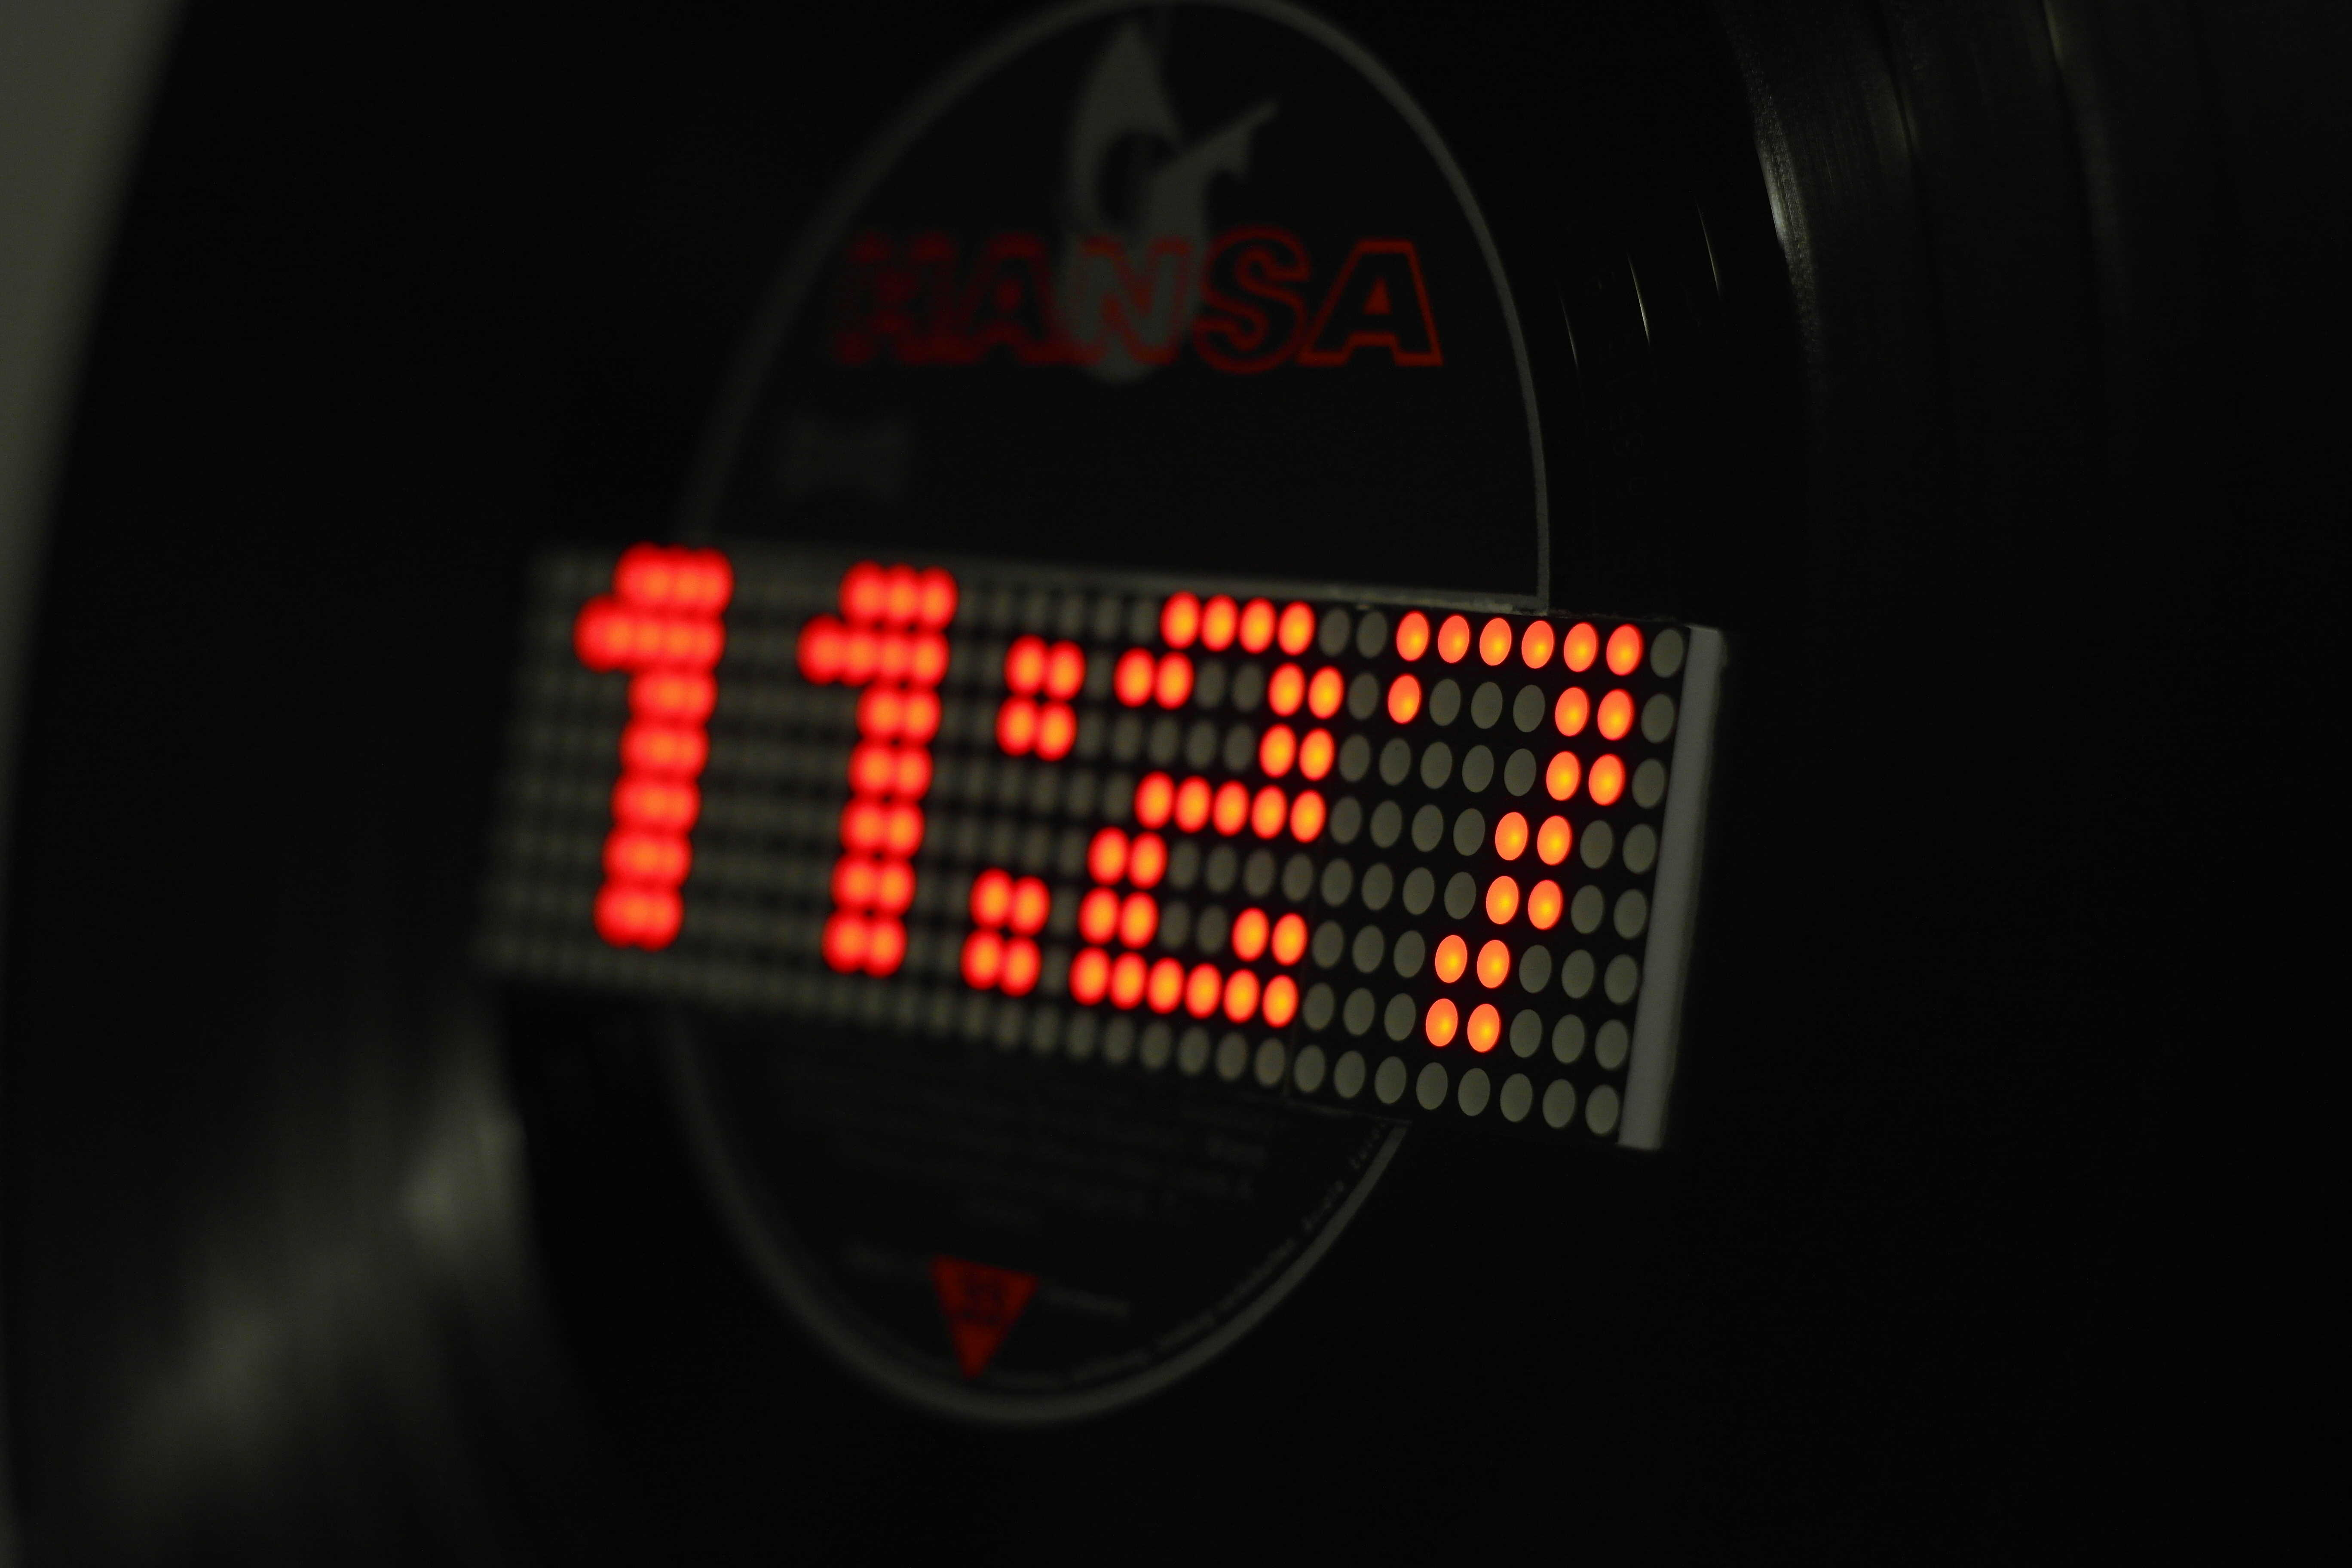
\includegraphics[width = 10cm]{images/clockface.JPG}
	\caption{Fénykép az óra számlapjáról}
	\label{fig:clockface}
\end{figure}	

Az óra számlapjának megjelenítéséhez szintén a kijelzőt reprezentáló mátrixot manipuláljuk.
Ebben az esetben fix pozíciókat használunk és a megjelenítendő számjegyek mátrixképei azonos szélességűek.
Az óra számjegyeihez egy külön karakterkészletet definiáltam, amelyek 0-9-ig reprezentálják a számokat. Ennek csupán esztétikai jelentősége van, a számjegyek a már meglévő karakterektől vastagabbak.
Az óra számlapja 4 számjegyből áll és a középen elhelyezkedő kettőspontból.
A 10-nél kissebb számjegyek elé egy nullást illesztünk, hogy a megjelenített kép szimmetrikus legyen.

\subsection{Vezetéknélküli kommunikáció}
Az eszközön megjelenő szöveget saját hálózaton keresztül van lehetőségünk küldeni. Az eszköznek csatlakoznia kell a felhasználó hálózatára. Ez WIFI kommunikációs protokollon valósul meg. A csatlakozást követően az eszköz a routertől kap egy saját IP címet és a 80-as portján egy HTTP szervert szolgáltat.
A szerveralkalmazás rendkívül egyszerű. Két kérést vesz vigyelembe: a GET, illetve a POST kéréseket.
Ezen kérések aszinkron léphetnek fel. Így a kérések beérkezésekor az üzenetet el kell tárolnunk egy \textit{bufferben}. Ha az ütemező a szervernek adja a futási jogot, az már a buffer tartalmát dolgozza fel.
A programomban egyetlen buffert használok. Ez problémát jelentene akkor, ha egyszerre több kérés érkezne be. Ilyenkor szerencsésebb lenne egy ún. körkörös buffer használata. De mivel az eszköz otthoni használatra lett tervezve, amelynek hálózatán kevés kliens van jelen, így egy buffer is elegendő a feladathoz.

\begin{figure}[ht]
	\centering
	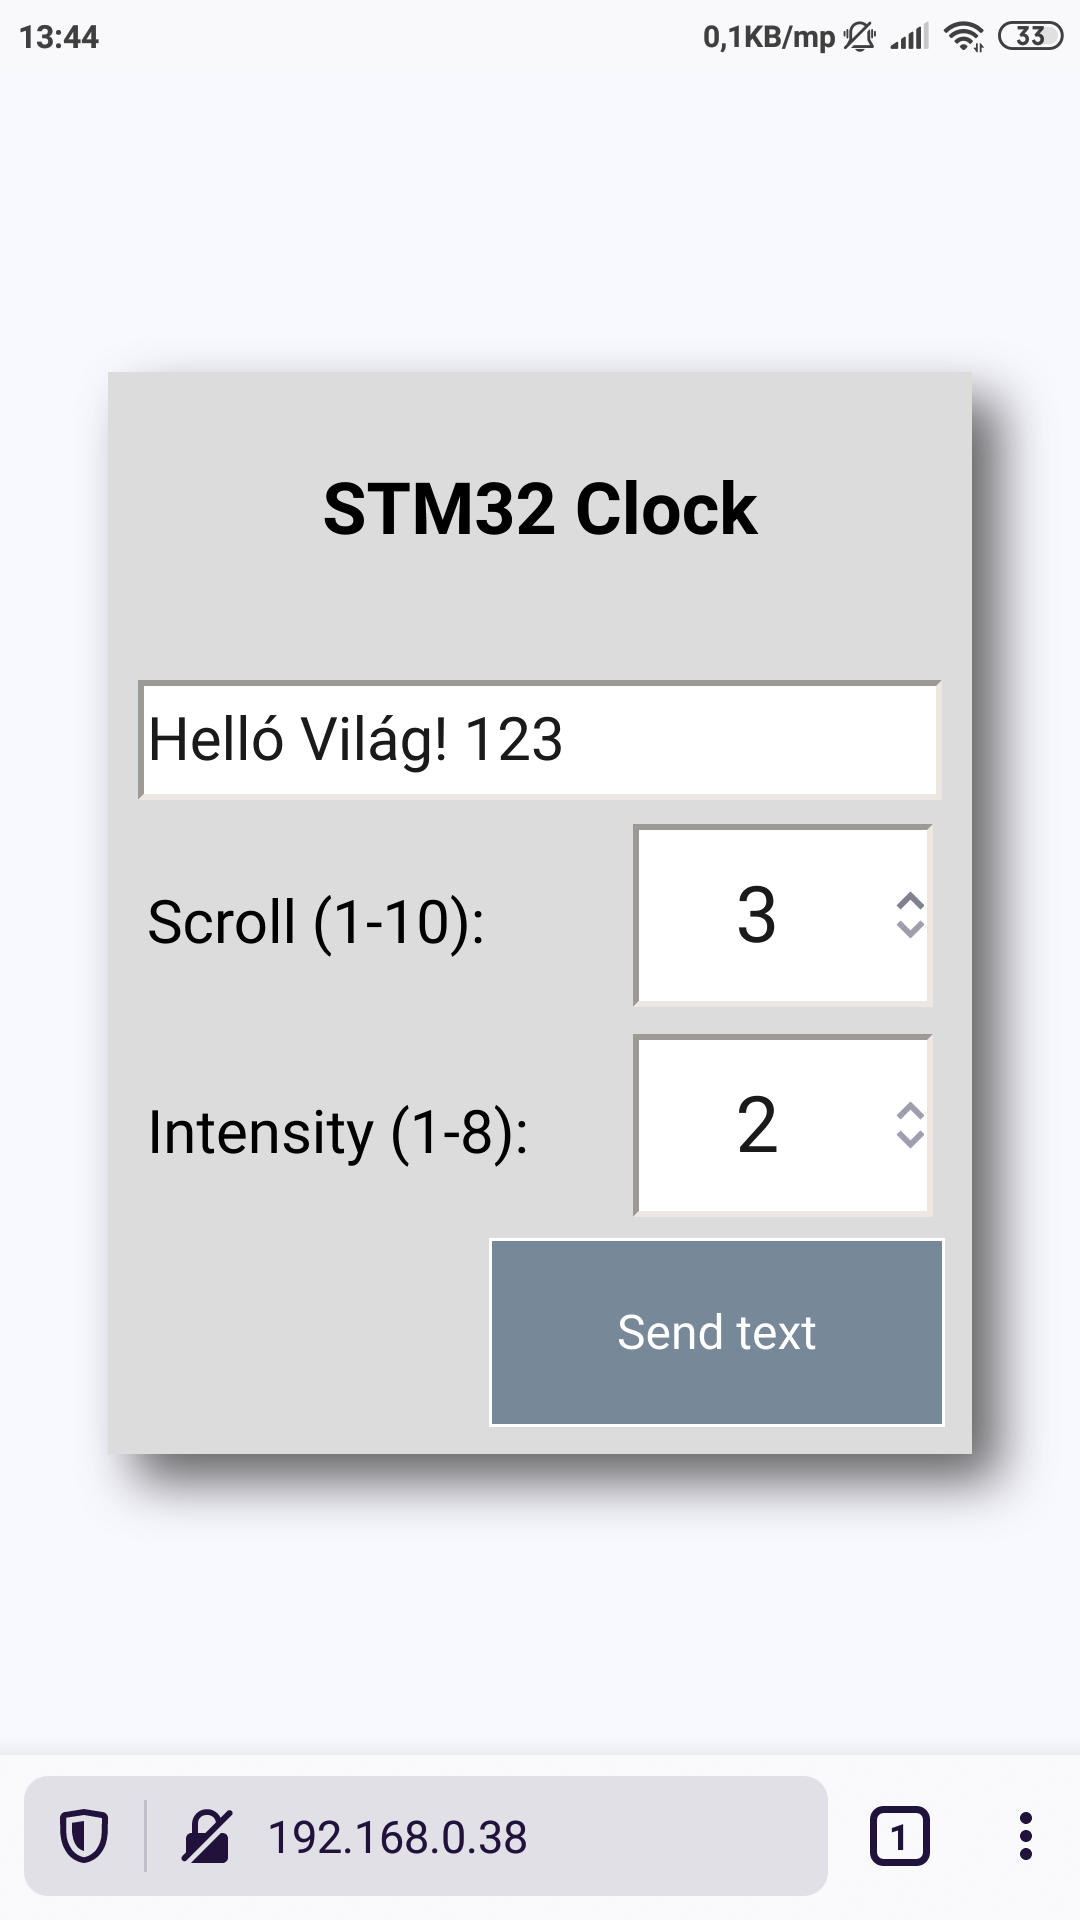
\includegraphics[width = 7cm]{images/webpage.png}
	\caption{Képernyőfotó a weblapról (\textit{Mozzilla böngésző, Android})}
	\label{fig:webpage}
\end{figure}	

\subsubsection{GET}

GET kérés esetén feltételezhetjük, hogy a kérés a weboldal betöltésére irányul, egy böngészőablakból. A kéréshez minden esetben tartozik egy \textit{link ID} is, vagyis egy azonosító, amely a kiszolgálásra váró klienst jelöli. A kérés feldolgozásakor az eszköz kiküldi a weboldalt a kliensnek. A weboldal tartalma egy inputmező, amelyben a kliensek szöveget írhatnak. Az inputmező alatt a kliens megadhatja, hogy a szövege hányszor csússzon végig a kijelzőn (\textit{Scroll times}), illetve a kijelző fényerejét is beállíthatja (\textit{Intensity}) a szövegküldéssel egyidejűleg.

\subsubsection{POST}

POST kérés esetén feltételezhetjük, hogy a kérés törzse a kliens által küldött szöveget tartalmazza.
A kérésben elküldött üzenet nem csupán az általa megadott szöveget tartalmazza. A frontenden megjelenített beállítások (\textit{Scroll times, Intensity}) mellett a kliens eszközének ideje is küldésre kerül.
Az üzenet kezdetét egy \texttt{+MSG\~} előtag jelöli. Az üzenet tagjait egy-egy \texttt{\~} (tilde) választja el egymástól.

Az üzenet tartalma:
\begin{enumerate}[nolistsep]
 \item \textit{Scroll times}
 \item \textit{Intensity}
 \item A hét napjának sorszáma
 \item Aktuális hónap
 \item Aktuális nap
 \item Aktuális év
 \item Óra
 \item Perc
 \item Másodperc
 \item A kiírandó szöveg 
\end{enumerate}

Mint látható, az üzenet tartalmazza a pontos időt és a dátumot is. Vagyis az eszköz belső órájának szinkronizálása az üzenetküldésekkel valósul meg. A kiírandó szöveg az utolsó tagként van jelen az üzenetben. Ennek két oka van: Ha a szöveg nem az utolsó tag lenne és a kliens tilde jeleket is elhelyezne a szövegben, akkor a feldolgozás során nem várt eredmény születne. A másik ok, amiért a szöveg az utolsó tag, mert ilyenkor akár üres szöveget is küldhetünk. Ilyen esetben megvalósul az óra szinkronizációja, beállításra kerül a kijelző fényereje és az eszköz nem vált át csúszó szöveges megjelenítésre.

\subsection{Időzítők}

Az alábbi időzítők megszakításokat generálnak. A megszakítások jelzésére egy-egy változó szolgál. Ha megszakítás következik be, a megfelelő változó 1-es (igaz) értéket vesz fel. A megszakításokat jelző változóknak az ütemezésnél lesz szerepük.

\subsubsection{Csúszó szöveg időzítő}
A szöveg kijelzésének folyamatában ismertetett $t$ időegységet jelenti. Megfigyeléseim szerint a 25Hz-es (40ms) időzítés megfelelő eredményt ad. Ezzel az értékkel a szöveg kijelzése se nem lassú, se nem gyors. Így a felhasználónak nincsen lehetősége továbbiakban ezt az értéket konfigurálni.

\subsubsection{Óra számlap frissítő időzítő}
A másik időzítő az óra képének kijelzésére szolgál. Ehhez egy 1Hz-es (1s) időzítőt használok. A megjelenítés szempontjából elegendő lenne egy lassabb időzítő is, hiszen a kijelző megtartja a beállított képét. Az egymásodperces időzítőt azért gondoltam idokoltnak, mert így az óra képének változása viszonylag gyorsan kijelezhető az aktuális időtől függetlenül.
Ha a frissítés pillanatában a másodperc 00 vagy 30 értékkel rendelkezik, akkor a számlap frissítése után egy kiírandó szöveg generálódik. Ilyenkor a kijelzőn csúszó szövegként a dátum és a hét napjának neve íródik ki.

\subsection{Real Time Clock}
Az pontos idő nyilvántartását egy RTC modul végzi. Az általam választott fejlesztői kártyán alapból megtalálható.
Az idő frissítése a kliensek által küldött szövegekkel együtt történik.

Az idő szinkronizációjára egy másik módszer lehet az NTP (\textit{Network Time Protocol}) szerverek használata. Viszont ez a lehetőség abban az esetben működne, ha az eszköznek minden szinkronizációs időben lenne internetelérése és a megadott NTP szerverek valamelyike működne.
Mivel a kliens által küldött időinformáció egyszerűbb és biztosabb, ezért az NPT szerveres szinkronizációt elvetettem.

\subsection{Ütemezés}
Az ütemezés Round-robin(kerge rigó) alapú. Egy előre meghatározott sorrend alapján működik a rendszer. A sorrend a következő:
\begin{enumerate}
	\item Szerver
	\item Csúszó szöveg frissítés
	\item Óra számlapjának frissítése
\end{enumerate}
Az ütemezésben a különféle megszakításoknak is kulcsszerepük van.

A szerveralkalmazás csak akkor kezdi el feldolgozni a kéréseket tartalmazó buffer tartalmát, ha annak hossza legalább 1. Ha az ütemező neki osztja ki a futási jogot és ez a feltétel teljesül, akkor először is egy kis ideig várakozik, hogy a kérés egésze beérjen a bufferbe. Ehhez egy előre meghatározott késleltetést adtam meg, ami alatt nagy valószínűséggel beérkezik a teljes üzenet. Ezután a buffer tartalmát feldolgozza a program és a tartalma alapján vagy kiszolgálja a klienst vagy lekezeli a POST kérést. Az üzenet feldolgozása után a buffer tartalma törlésre kerül, hossza így 0 lesz, és a következő üzenet beérkezéséig a futási jogot egyből átadja a soron következő kódrészletnek.

Ha az ütemezés a csúszó szöveg frissítésére esik, akkor elsősorban le kell ellenőrizni, hogy van-e kiírandó szöveg. A másik feltétel pedig a szövegfrissítő időzítő megszakításának jelzésének \textit{igaz} értéke. Ha teljesülnek a feltételek, akkor a már ismertetett módon egy lépéssel frissíti a kijelző mátrixát, \textit{hamis} értékre állítja a megszakítás jelzésére szolgáló változót és a futási jogot a soron következőnek adja.

Az ütemezés utolsó résztvevője az óra számlap frissítő kódja. Ha az óra számlapjának időzítője megszakítást generált, vagyis a megszakítás figyelő változó \textit{igaz} értékkel rendelkezik és nincsen kiírandó szöveg, akkor kirajzolódik az óra számlapja. Félpercenként csúsztatni való szöveg is generálódik, amely az aktuális dátumot és a nap nevét tartalmazza. A műveletek végén a megszakítás jelzéséért felelős változót \textit{hamisra} állítja.

\section{Megvalósítás}
\subsection{Felhasznált hardverek}

\begin{figure}[ht]
	\centering
	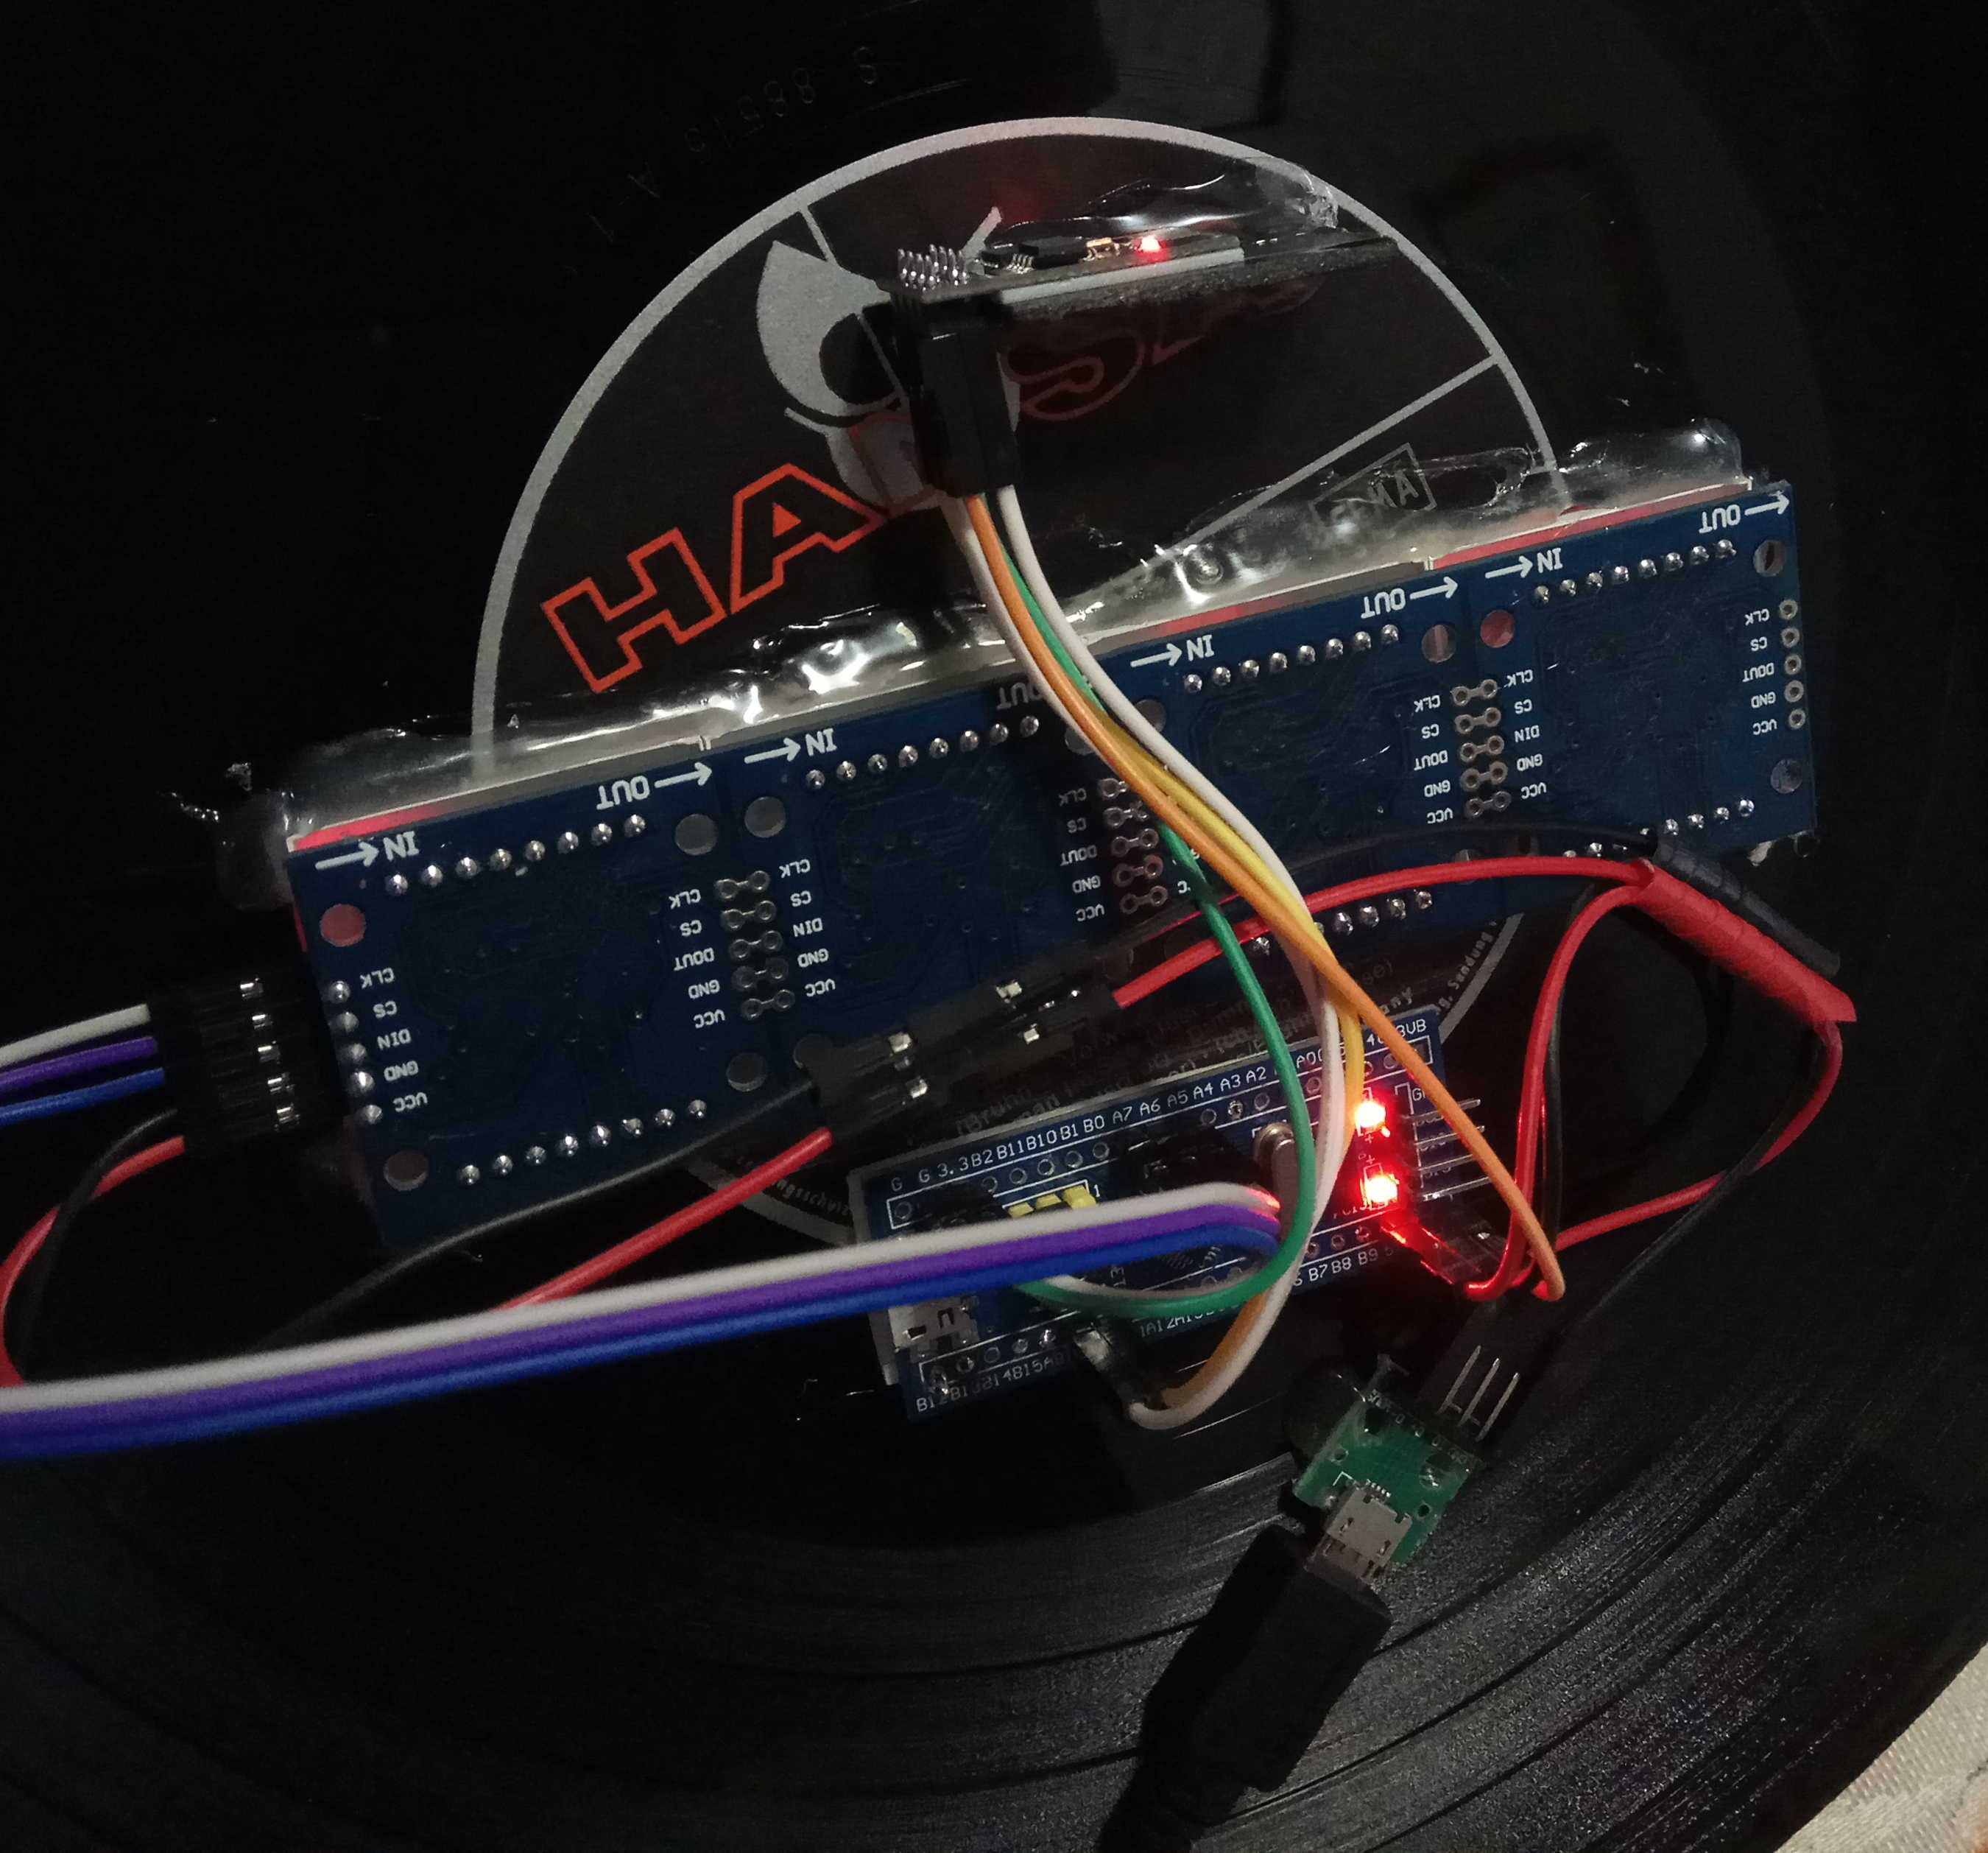
\includegraphics[width = 12cm]{images/back.jpg}
	\caption{Az elkészült feladat hátoldala}
	\label{fig:back}
\end{figure}

Az elkészült feladat vázát egy bakelit lemez adja (Manuela: Die großen Erfolge). A lemez címkéjénél a kijelző méretével megegyező lyukat vágtam ki. Így előlről nézve csak a kijelző felülete látszódik, a többi alkatrész takarásban van. A hardverek a lemez hátoldalán vannak elhelyezve. A fejlesztői kártya és a Wifi modul kétoldalú ragasztóval van rögzítve, a kijelző és a micro USB aljzat pedig hőre lágyuló ragasztóval. 

\subsubsection{STM32F103C8T6 fejlesztői kártya}
Az általam elkészített feladat alapja az \texttt{STM32F103C8T6} fejlesztői kártya, amelyen egy ARM 32-bit-es mikrovezérlő helyezkedik el. Cortex-M3-as processzorral rendelkezik és 72 MHz maximum frekvenciával képes működni. 64 Kbyte Flash memóriával és 20 Kbyte SRAM-al (\textit{Static RAM}) rendelkezik. A programom a CUBE IDE szerint 24.73 KB Flash memóriát és 4.88 KB RAM-ot foglal le ebből.
A fejlesztői kártyán megtalálható egy beépített RTC (\textit{Real Time Clock}) egység is, amely az idő számolását végzi a háttérben.

\begin{figure}[ht]
	\centering
	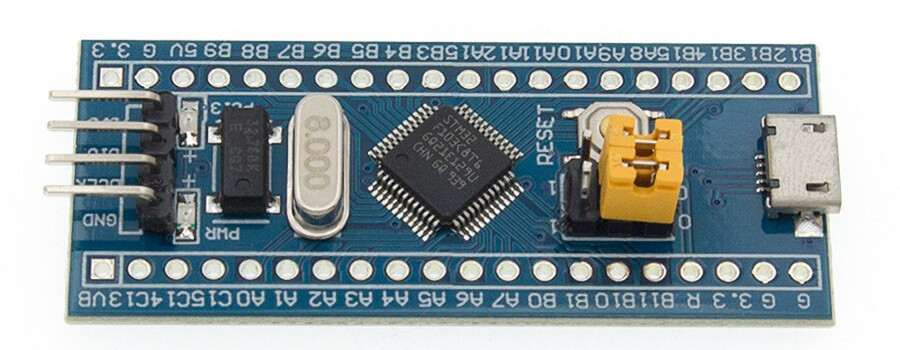
\includegraphics[width = 9cm]{images/stm32.jpg}
	\caption{A fejlesztői kártya}
	\label{fig:mcu}
\end{figure}

\begin{center}
\begin{tabular}{ | l | l | }
\hline
\multicolumn{2}{|c|}{\textit{\Large{A használt pinek}}} \\
\hline
\textbf{PIN} & \textbf{Funkció}\\
\hline
5V & Bemeneti feszültség\\
G & A tápegységtől kapott Ground\\
\hline
A5 & Csatlakozás a LED driver CLOCK pinjére\\
A6 & Csatlakozás a LED driver CS pinjére\\
A7 & Csatlakozás a LED driver Data pinjére\\
\hline
A10 & USART RX, amely az ESP-01 TX pinjére csatlakozik\\
A9 & USART TX, amely az ESP-01 RX pinjére csatlakozik\\
G & Csatlakozás az ESP-01 Ground pinjéhez\\
3.3V & Az ESP-01 áramellátása, csatlakozás a VCC pinjéhez\\
3.3V & Csatlakozás az ESP-01 CH\_EN pinjéhez\\
\hline
\end{tabular}
\end{center}

A kártya programozásához szükségünk van egy külső eszközre, egy programozóra, mivel a kártyán nem található ilyen. Az általam használt programozó az \texttt{ST-Link V2}, amelyet USB porton csatlakoztathatunk a számítógéphez. A fejlesztői kártyához az SWDIO, GND, SWCLK és a 3.3V-os pinekkel csatlakozhatunk.

\begin{figure}[ht]
	\centering
	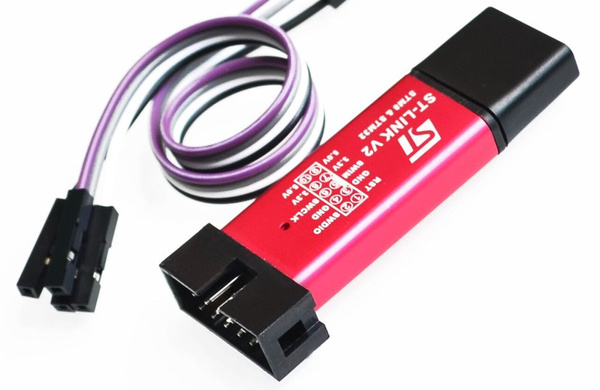
\includegraphics[width = 8cm]{images/stlink.jpg}
	\caption{A programozó}
	\label{fig:stlink}
\end{figure}	

A fejlesztői kártyán egy \textit{jumper} segítségével választhatjuk ki a futási és programozási módot. A CUBE IDE-ben a megfelelő beállítások alkalmazásával nem szükséges a jumpert átrakosgatni a programozáskor, maradhat futási módban, ezzel is meggyorsítva a fejlesztést.

\subsubsection{ESP-01 (ESP8266)}
Az \texttt{ESP-01} valójában szintén egy mikrovezérlő, de a projektemben WIFI modulként használtam fel, vagyis ez felel a vezetéknélküli kommunikációért. 802.11 b/g/n szabvánnyal rendelkezik, 2.4 GHz-es csatornát használ. Támogatja a WPA/WPA2-t, és tud működni Station és Access Point módban is.

A fejlesztői kártyával USART kommunikációs protokollon keresztül kommunikál. A modul működtetéséhez az általa ismert AT parancsokat kell továbbítanunk. Áramellátását az STM32 kártyától kapja.

\begin{figure}[ht]
	\centering
	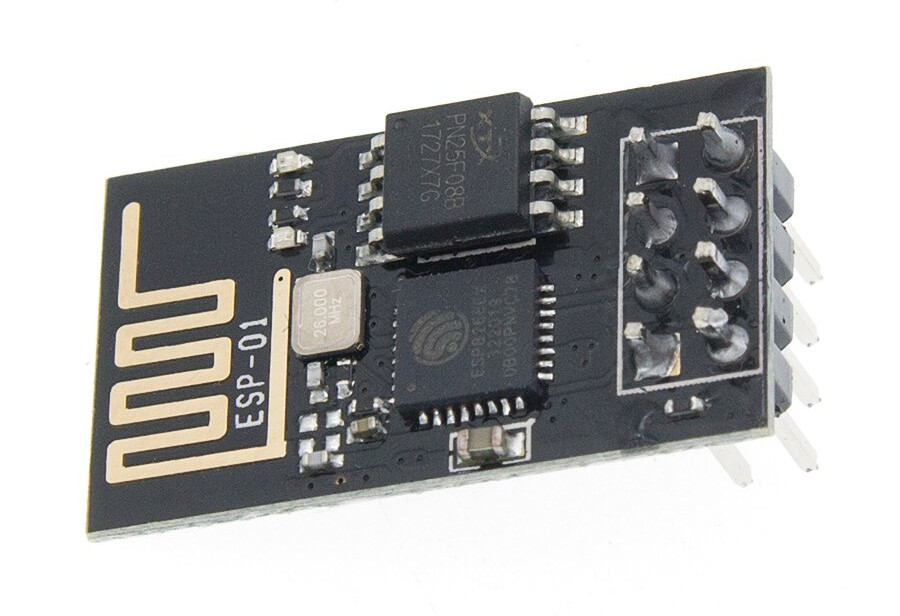
\includegraphics[width = 6cm]{images/esp01.jpg}
	\caption{A Wifi modul}
	\label{fig:esp01}
\end{figure}	

\subsubsection{MAX7219-4DM}
A kijelző 4 db 8x8-as LED mátrixból áll, amely mögött 4 db MAX7219 LED meghajtó üzemel. Ezt az összekaszkádolt kijelzőt készen rendeltem az internetről, mivel a tulajdonságai alapján teljesen megfelelt az elképzeléseimnek. A 4 db mátrix tökéletesen alkalmas egy digitális óra 4 számjegyének megjelenítésére, és a csúsztatott szöveg kijelzése is megoldható vele, hiszen a 4 mátrix megfelelő szélességű felületet biztosít a szavak kirajzolásához.
A kijelző működtetéséhez 5V kell. Ezt a tápegységtől kapja meg. A kijelzéshez szükséges jeleket a fejlesztőikártya 3 különböző GPIO portjától kapja meg.

\begin{figure}[ht]
	\centering
	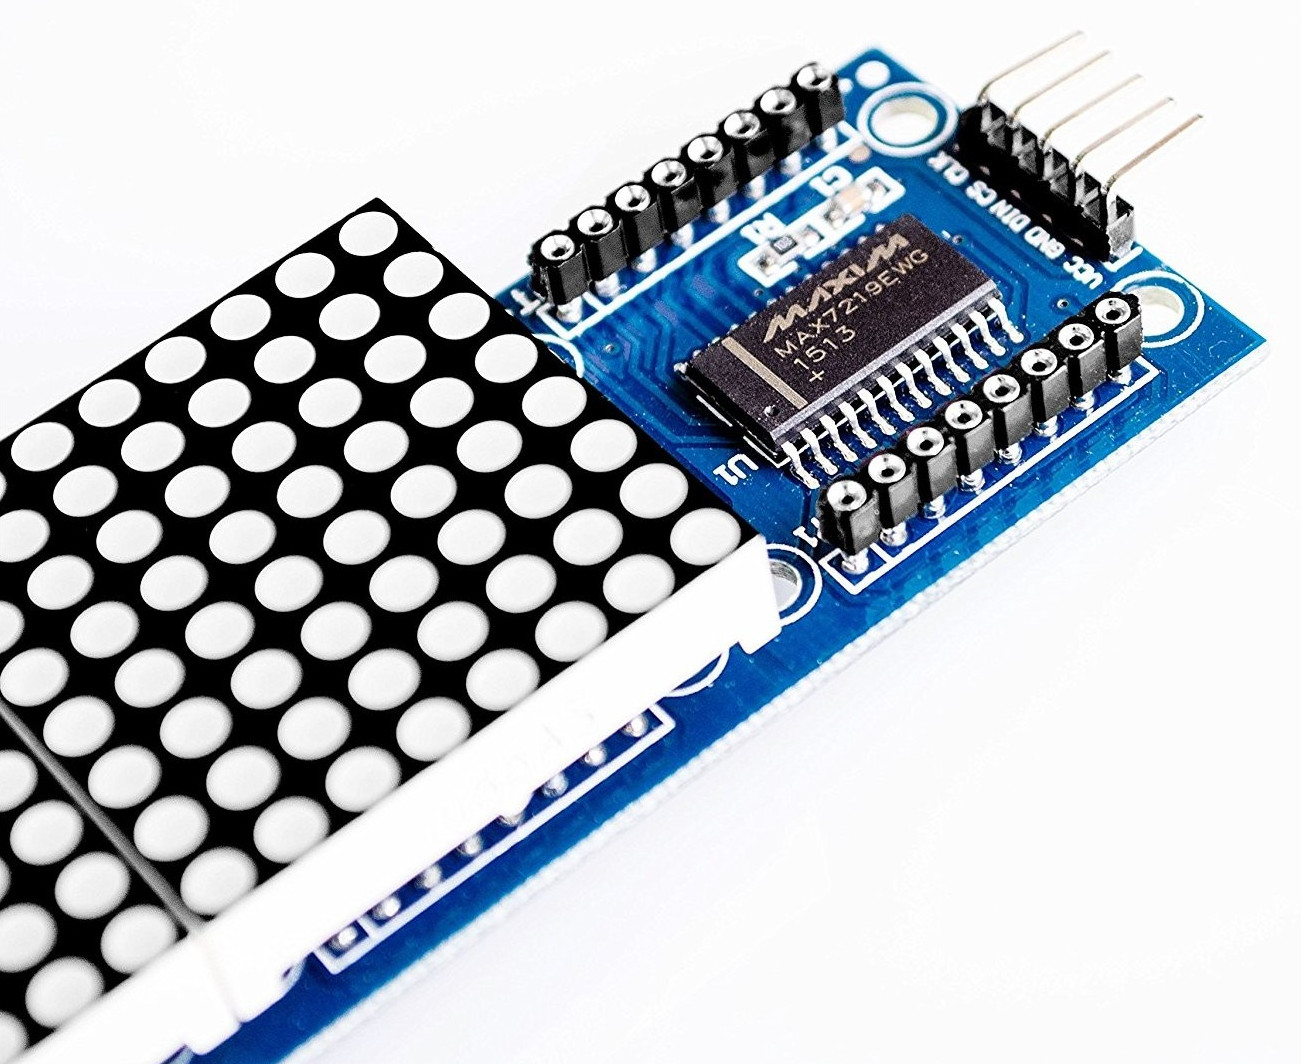
\includegraphics[width = 8cm]{images/matrix.jpg}
	\caption{A kijelző és a LED meghajtó}
	\label{fig:matrix}
\end{figure}	

\subsubsection{Micro USB aljzat + Tápegység}

Az eszközön helyet kapott egy micro USB aljzat is, amelynek a GND és a VBUS kimeneti pinjeit használtam fel. A fejlesztői kártyához és a kijelzőhöz csatlakozik párhuzamosan.

\begin{figure}[ht]
	\centering
	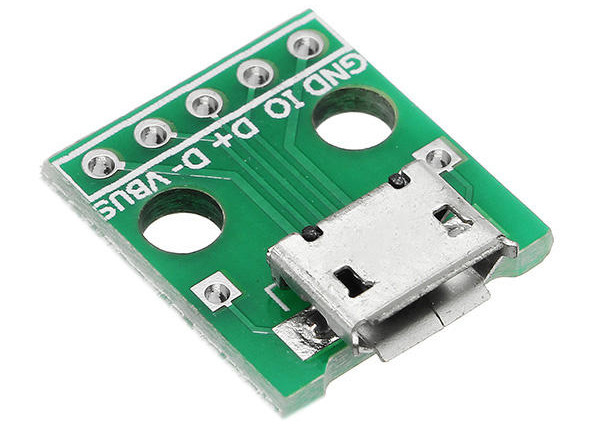
\includegraphics[width = 5cm]{images/dip5.jpg}
	\caption{Micro USB aljzat}
	\label{fig:dip5}
\end{figure}

Az általam használt tápegység (\texttt{JX-005}) pedig 5V-ot és 2 ampert tud leadni.

\subsection{A program}

A programot az \textit{STMicroelectronics STM32CubeIDE 1.4.0}-val írtam.
Az IDE által generált kódokon kívül a következő forrásállományokat hoztam létre:
\begin{itemize}[noitemsep]
	\item \texttt{max\_driver.c}
	\item \texttt{max\_display.c}
	\item \texttt{scrolling\_text.c}
	\item \texttt{clock\_face.c}
	\item \texttt{uart\_handler.c}
	\item \texttt{esp01.c}
\end{itemize}

\subsubsection{Megjelenítés}

A \texttt{max\_driver.c} tartalmazza az összes olyan metódust, amelyek a LED vezérlők működtetéséhez szükségesek.
A LED vezérlőegységeknek bájtok formájában küldhetünk adatokat.
Egy bájt elküldése a következőképpen tehető meg:
\begin{lstlisting}[style=CStyle]
void write_byte (uint8_t byte){
	for (int i = 0; i<8; i++){
		HAL_GPIO_WritePin (MAXPORT, CLOCK_PIN, 0);
		HAL_GPIO_WritePin (MAXPORT, DATA_PIN, byte&0x80);
		byte = byte<<1;
		HAL_GPIO_WritePin (MAXPORT, CLOCK_PIN, 1);
	}
}
\end{lstlisting}
Mint látható, a bájtot bitenként küldhetjük el. Minden bit elküldésénél a kijelző óra pinjét le kell húznunk, az adat pinjén beállítjuk a megfelelő bit értékét, majd az óra pinjét felhúzzuk. Ezt addig ismételjük, amíg a teljes bájtot át nem küldtük.

A vezérlő értékeit a megfelelő regiszterek címzésével állíthatjuk be.

Első lépésként a kijelző CS pinjét le kell húznunk, majd a kiválasztott regiszter számát kell elküldenünk a már ismert módon. Ezután a regiszterbe küldendő bájtot kell továbbítanunk. Végül a CS pint előbb 0-ra, majd 1-re húzzuk fel.

A vezérlő konfigurálásához dedikált vezérlők állnak rendelkezésre. A kijelző inicializálása ezen regiszterek beállításával történik a \texttt{void max\_init(uint8\_t intensity)} függvénnyel.

A $8\times 8$-as mátrix értékeit soronként adhatjuk meg a megfelelő bájtok beállításával. A sorok regisztercímei 1-8 ig terjednek.

Mivel a kijelző LED vezérlők és mátrixok kaszkádolásából áll, így a soroknak elküldött értékek minden cellábban ugyan azok a LED-ek villannak fel. A megfelelő cella kiválasztásához meg kell adnunk a cella indexét. Az indexelés 0-tól kezdődik. Amíg el nem érjük a kívánt cellát, addig az előtte lévő cellákat a 0 című regiszter 0 értékének beállításával léphetjük át. Majd ha elértük a cellát, a megfelelő sorát elláthatjuk a bájt értékével. Ezután a maradék cellákat is a 0,0 értékkel kell ellátnunk. A műveletet a \texttt{void set\_byte\_on\_matrix(uint8\_t byte, uint8\_t row, uint8\_t column)} függvénnyel tehetjük meg.

\bigskip

A \texttt{max\_display.c}-ben található meg a kijelző reprezentálására szolgáló \texttt{screen\_buffer}, amely egy kétdimenziós mátrix. 8 sorral rendelkezik és annyi oszlopa van, ahány cella van a kijelzőben.
A forrásállomány ezen mátrix manipulálására szolgáló metódusokat tartalmaz, illetve itt kap helyet a már említett karakterkészlet is.

\bigskip

A \texttt{scrolling\_text.c} állományban találhatóak meg a csúszó szöveg megjelenítésért felelős eljárások.

\noindent Mindkét függvény ugyan azt az eredményt szolgáltatja, viszont a \texttt{void scroll\_text\_left\_IT (Scrolling\_text* st)} megszakítás alapú, míg a másik belső késleltetéseket használ. Az utóbbi az eszköz inicializálásánál van szerepe, hiszen ilyenkor még nem léptünk be a főciklusba, így elengedhetetlen a soros működés.

A megszakítás alapú kiíratás csúszó szövegét az alábbi struktúrával adhatjuk meg:
\begin{lstlisting}[style=CStyle]
typedef struct Scrolling_texts {
   char text[600];
   int times;
   int char_index;
   int char_column;
} Scrolling_text;
\end{lstlisting}
A \texttt{text} adattagban helyezkedik el a kiírandó szöveg. A \texttt{times} az ismétlés számát adja meg. A \texttt{char\_index} és \texttt{char\_column} pedig a \ref{csuszo} fejezetben már ismertetett csúszó szöveg kiíratásában szereplő $i$ és $j$ értékek. 

\bigskip

A \texttt{clock\_face.c} forrásállomány az óra számlapjának megjelenítésére szolgáló két metódust tartalmazza.

\subsubsection{Wifi kommunikáció}

Az \texttt{uart\_handler.c} csupán azokat az UART kezelő függvényeket tartalmazza, amelyek a soros működésű UART kommunikációban használatosak. Ilyen soros működésre van szükség például az ESP-01 inicializálása során is, illetve az UART-on való küldés is minden esetben soros működésű.

\bigskip

Az \texttt{esp01.c} két metódust tartalmaz: az inicializáló metódusát, amely az eszköz beállítására szolgál és a szerverkezelő metódust.
Az ESP-01 modul működtetéséhez ún. AT parancsokat kell küldenünk. Ezeket a parancsokat a kártya értelmezi és a bennük található utasításokat végrehajtja.

Az eszköz inicializálásához elegendő megadnunk a Wifi hálózatunk SSID-jét és jelszavát. Az eszköz ezután megpróbál csatlakozni rá. Ezt a következőképpen tehetjük meg:
\begin{lstlisting}[style=CStyle]
char* device_ip = esp_init("ssid", "pswd");
\end{lstlisting}
Az inicializáló függvény visszatérési értéke a routertől kapott lokálishálózatos IP címe. Ezen cím 80-as portján az eszköz egy HTTP szervert szolgáltat.

\subsubsection{Megszakítások}

A megszakítások jelzésére a már ismertetett változók szolgálnak.

Az eszköz működése során az UART kommunikáció is generál további megszakításokat.
A programban a főciklusba lépés előtt az UART kommunikáció átvált asszinkron módra. Bejövő adat esetén karakterenként újjabb megszakítás generálódik. A megszakítás lekezelése után a kapott karaktert egy bufferben helyezem el, növelem a karakterszámláló értékét, majd újra elindítom az asszinkron UART figyelőt.
Az \texttt{stm32f1xx\_it.c} UART megszakításkezelőjét a következőkkel egészítetem ki: 
\begin{lstlisting}[style=CStyle]
void USART1_IRQHandler(void)
{
  /* USER CODE BEGIN USART1_IRQn 0 */
	uart_interrupt = 1;

  /* USER CODE END USART1_IRQn 0 */
  HAL_UART_IRQHandler(&huart1);
  /* USER CODE BEGIN USART1_IRQn 1 */
	receive_buffer[uart_interrupt_counter] = receive_it;

	uart_interrupt_counter++;

  HAL_UART_Receive_IT(&huart1, &receive_it, 1);

  /* USER CODE END USART1_IRQn 1 */
}
\end{lstlisting}

\subsubsection{A főciklus}

A \texttt{main.c}-ben található meg a program végtelen ciklusa. Itt kap helyet a már ismertetett Round-robin ütemező is.

\begin{lstlisting}[style=CStyle]
while (1)
{
	if(uart_interrupt && uart_interrupt_counter > 1){
		/* Server */
	}
	if(update_screen == 1 && strlen(scrolling_text.text) != 0){
		/* Updating the scrolling text */
	}
	if(update_clock == 1 && strlen(scrolling_text.text) == 0){
		/* Updating the clockface */
	}
}
\end{lstlisting}

\section{A kódbázis elérhetősége}
Az eszköz programjának a kódja az alábbi repositoryban érhető el:\\
\url{https://github.com/DanielNagy97/embedded2020}

\end{document}
